\chapter{Communication}

It is desirable that the system can be controlled from a user interface. The development board supports a OLED display, and two buttons that can be used to interact with the system, but to add more flexibility to the user interface, a GUI is designed on a PC. To data exchange between the DSP and a PC a communication interface is needed. The DSP has an UART hardware device and is chosen to be used as the communication interface. 

\section{Communication between DSP and PC}

As PC's usually do not have a serial port for UART interfacing, a converter is needed.   

\begin{figure}[H]
\centering
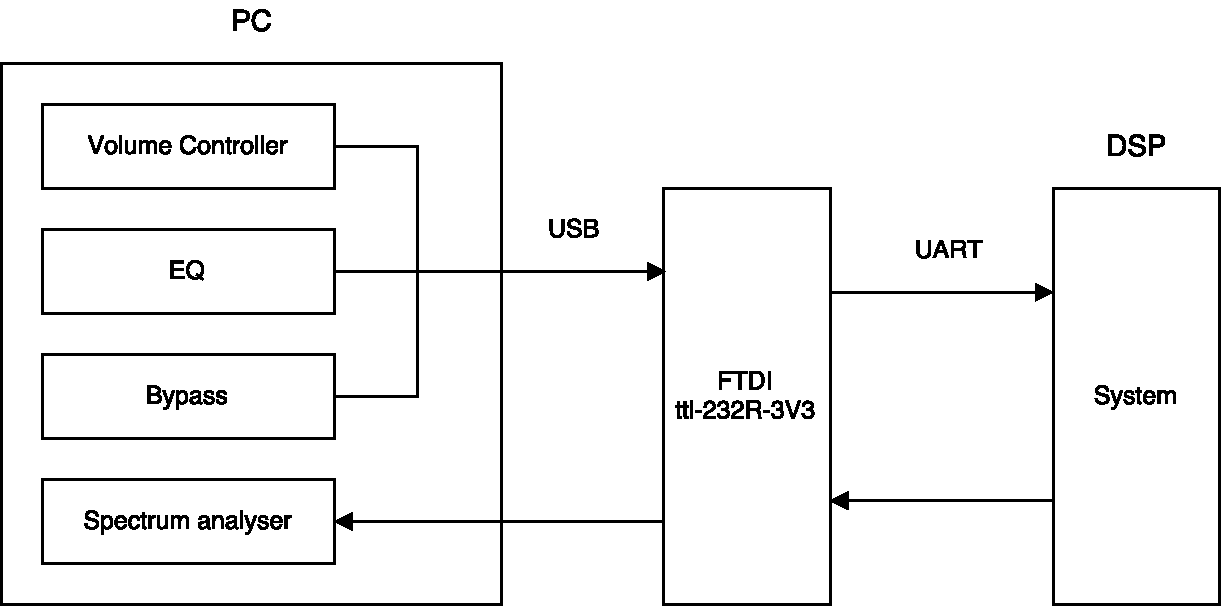
\includegraphics[width=0.75\textwidth]{figures/communicationBlock.pdf}
\caption{Overview of the interface with the DSP.}
\label{fig:communicationBlock}
\end{figure}


\begin{figure}[H]
\centering
\begin{subfigure}[t]{0.47\textwidth}
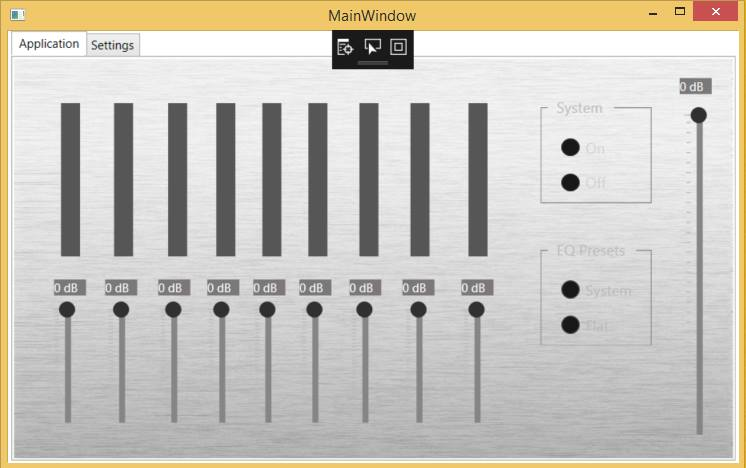
\includegraphics[width=\linewidth]{GUIApp}
	\caption{Group delay of a 4th order IIR filter.}
	\label{fig:GUIApp}
\end{subfigure}
\hspace{6mm} 
\begin{subfigure}[t]{0.47\textwidth}
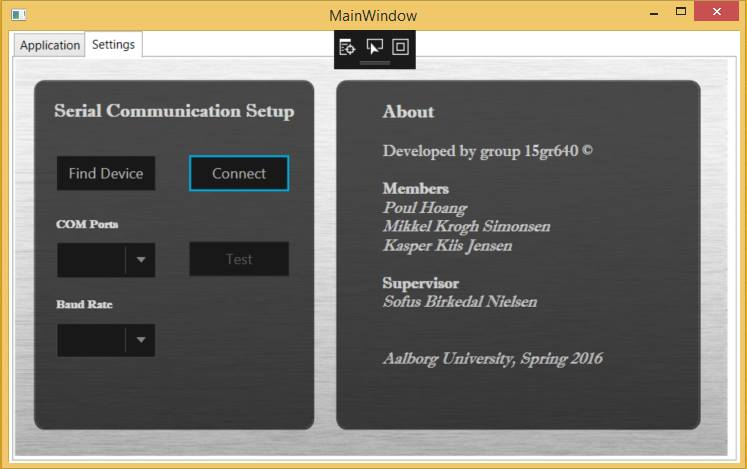
\includegraphics[width=\linewidth]{GUISettings}
	\caption{Group delay of a 50th order FIR filter.}
	\label{fig:GUISettings}
\end{subfigure}
\caption{Group delay of IIR and FIR filter.}
\label{fig:GUI}
\end{figure}

\section{Volume Controller, Equalizer and Bypass}

\begin{figure}[H]
\centering
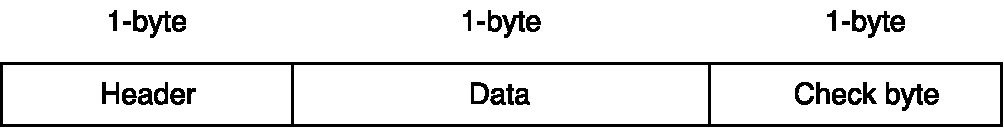
\includegraphics[width=0.75\textwidth]{figures/communicationProtocolUART.pdf}
\caption{Overview of the interface with the DSP.}
\label{fig:communicationProtocolUART}
\end{figure}



\begin{lstlisting}[language=C, caption = {Delay function for bypass},label={listingByPass}]
int16 delayBypass(int16 dataIn, int16 *dataBuffer, int16 *dataPtr){
	int16 temp;
	temp = dataBuffer[*dataPtr];
	dataBuffer[*dataPtr] = dataIn;
	(*dataPtr)++;
	if (*dataPtr == 5333){
		*dataPtr = 0;
	}
	return temp;
}
\end{lstlisting}

\section{Spectrum Analyser}

\begin{figure}[H]
\centering
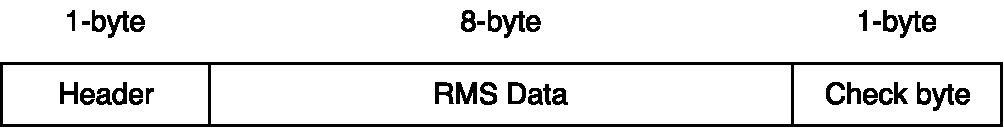
\includegraphics[width=0.75\textwidth]{figures/communicationProtocolUARTTransmit.pdf}
\caption{Overview of the interface with the DSP.}
\label{fig:communicationProtocolUARTTransmit}
\end{figure}


\begin{lstlisting}[language=C, caption = {Calculate RMS value},label={listingRMSuart}]
uint8 RMScalculate(int16 *dataBuffer, int16 dataIn, int16 *BufferPtr, long *sum){
	// Initialize local variables
	uint8 result; long temp;
	
	// Calculate RMS^2
	*sum = *sum - dataBuffer[*BufferPtr]; // Substract the oldest data from sum
	temp = (long)dataIn*dataIn;	// Square the new sample
	dataBuffer[*BufferPtr] = temp>>15;	// Bit-shift and store in data buffer
	*sum = *sum + dataBuffer[*BufferPtr];
	result = ((*sum)>>4)>>5;				// Calculate new RMS^2
	
	// Increment data pointer
	(*BufferPtr)++;
	if (*BufferPtr == 16){ 
		*BufferPtr = 0;
	}
	
	return result;
}
\end{lstlisting}
\todo[inline]{Fejl i koden! BufferPtr skal sammenlignes med 32 og ikke 16! Samt bit shift på 10 og ikke 9.}



% Appendix - Baudrate, register setup. Husk external bus setup.

